\documentclass{article}

\usepackage[utf8]{inputenc}
\usepackage[T1]{fontenc}
\usepackage{lmodern}

\usepackage{parskip}
\usepackage{graphicx}
\usepackage{tikz} 
\usepackage{xcolor} 
\usepackage{mathrsfs}
\usepackage{stmaryrd}
\usepackage{amssymb}
\usepackage{cancel}
\usepackage{amsthm,amsmath}
\usepackage{mathtools}
\usepackage{mdframed}
\usepackage{pgfplots}
\usepackage{float}
\usepackage{needspace}
\usepackage{listings}
\usepackage{subcaption}
\usepackage{csquotes}

\usepackage[normalem]{ulem} 

\usepackage{url}
\usepackage{hyperref}
\hypersetup{
    colorlinks=false,
    linkcolor=black,
    filecolor=black,      
    urlcolor=black,
}

\usepackage[
    backend=biber,
    style=numeric,
    sorting=none
]{biblatex}
\addbibresource{references.bib}

\usepackage[margin=3.5cm]{geometry}
\pgfplotsset{compat=1.18}
\usepgfplotslibrary{polar}

\renewcommand{\proofname}{Proof}

\setcounter{tocdepth}{2}
\renewcommand{\contentsname}{Table of contents}
\newmdenv[
    linewidth=1pt,
    roundcorner=5pt,
    linecolor=black,
    frametitle={Definition}
]{definitionbox}
\newmdenv[
    linewidth=1pt,
    roundcorner=5pt,
    linecolor=black,
    frametitle={Theorem}
]{theorembox}
\newmdenv[
    linewidth=1pt,
    roundcorner=5pt,
    linecolor=black,
    frametitle={Property}
]{propertybox}
\newcommand{\remark}[1]{%
    \textbf{\textcolor{black}{Remark.}} #1%
}
\newcommand{\notation}[1]{%
    \textbf{\textcolor{black}{Notation.}} #1%
}

\newcommand{\corollary}[1]{%
    \textbf{\textcolor{black}{Corollary.}} #1%
}
\newcommand{\norm}[1]{\left\|#1\right\|}
\newcommand{\dotproduct}[2]{\langle #1, #2 \rangle}

\title{Study of the Cox-Ross-Rubinstein model for option valuation}
\author{Thomas Saurel}
\date{January 2026}

\begin{document}

\begin{titlepage}
    \centering
    \vspace*{4cm}
    
    {\Large \textsc{Thomas Saurel} \par}
    
    \vspace{2.5cm}

    \rule{0.6\textwidth}{0.4pt} \\ [0.5cm]
    {\Huge \bfseries Study of the Cox-Ross-Rubinstein model for option valuation \par}
    \vspace{0.3cm}
    \rule{0.6\textwidth}{0.4pt}
    
    \vfill
    
    {\large Started in January 2026 \par}
    {\small Last update : \today \par}
    
\end{titlepage}

\newpage
\tableofcontents
\newpage

\section{Introduction}
\vspace{0.5cm}
\begin{center}
    \textit{"A good portfolio is more than a long list of \\
    good stocks and bonds. It is a balanced whole $[...]$."}\\
    -- \textbf{H. Markowitz \cite{MarkowitzQuote}} --
\end{center}
\vspace{0.5cm}
    
\subsection{Motivation}
This document was made to be an introduction to quantitative finance through development of market risk analysis algorithms.
It focuses on the study of the binomial model, known as the Cox-Ross-Rubinstein model.

Firstly, we will talk about the theoretical foundations of this prediction model before analyzing how it differs from the Black-Scholes and Monte Carlo models.
Finally, we will implement and analyze the  market variation estimators, known as the "Greeks".

I am working on this paper in my spare time for personal learning and curiosity. Consequently, it may contain errors or inaccuracies. 
The provided sources are in French or English, you may use a translator if you do not understand either of these languages.

\subsection{History of option valuation}

Modern portfolio theory in finance originated in 1952 with the work published by Harry Markowitz \cite{HarryMarkowitz}.
This theory explains how investors can optimize their portfolios and analyze asset pricing based on market conditions (volatility, risk and so on). 
Therefore it lays the foundations of quantitative finance by defining the portfolio as a collection of financial assets.

Based on Markowitz's work, three economists \textit{Fischer Black}, \textit{Myron Scholes} and \textit{Robert Merton} published an article in 1973 presenting a formula allowing to calculate the theoretical price of a European option.
Their contribution was to find a partial differential equation (PDE) to find the fair price for a European call option. \cite{Option}

With the development of computers and the exponential growth of computing power, a new method emerged in 1977 : the Monte Carlo approach. 
This model involves randomly simulating thousands of possible price paths.
The option price is the the average of the payoffs obtained from these paths. \cite{MonteCarloPricing}
It is the primary method for exotic options such as Asian options, where the payoff depends on the average price over a certain period of time.\cite{AsianOption}

Two years later, a new trio of economists :  \textit{John Cox}, \textit{Stephen Ross} and \textit{Mark Rubinstein} proposed an innovative alternative : the binomial model, also known as the Cox-Ross-Rubinstein model.
In this model, time is discretized, allowing the path of an asset price to be represented as a binary tree.
This simplifies estimation, providing a numerical approximation to the Black-Scholes model which relies on an anlytical solution.
The approach shifts the problem from a complex partial differential equation to a simple approximation that can be programmed on a computer.
Furthermore, the model enables the valuation of American options, wich can be exercised at any time with only a minor change in the algorithm. \cite{OptionPricingASimplifiedApproach}

Subsequently, other more exotic models appeared (e.g. trinomial trees) \cite{TrinomialTree}.
In one of the following part, we will focus on the binomial model and compare it with the Black-Scholes and Monte Carlo models, representing respectively an approximation model, an analytical model and a simulation-based one.
The Cox-Ross-Rubinstein model is more intuitive and simpler to implement algorithmically than the Black-Scholes model.

\subsection{Goals}

The main goal of this paper is to present the theoretical foundations of the binomial model, implement it and the compare it to other option pricing models.

We will begin by establishing the basic terminology and presenting key theoretical results from financial mathematics.
Once the model's algorithmic implementation is complete, we will explore its capabilities by pricing complex options.
We will analyze how the model's discrete structure allows for the valuation of products that cannot be handled analytically by the Black-Scholes model, such as American options which can be exercised early.
The study will be complemented by the calculation of sensitivity indicators known as \textit{Greeks}, which are essential risk management tools for measuring a portfolio's sensitivity to market volatility.

Finally, we will compare our results with those obtained from the Black-Scholes and Monte Carlo models. 
This comparative analysis will enable us to highlight the binomial model's convergence rate and identiy its limitations when applied to real-world date, thereby preparing for potential extensions involving more sophisticated tree structures.

\subsection{Vocabulary}

Before proceeding with the study of quantitative finance and the algorithms behind the Cox-Ross-Rubinstein model, it is essential to establish a basic vocabulary necessary for a proper understanding of the remainder of the document. 
If you have a financial background, you can skip this part as it will only present the basic key ideas in market finance.


\underline{\textbf{Derivative :}} A derivative is a type of financial contract whose value depends on an asset known as \textbf{underlying asset} and whose price fluctuates in line with changes in the rate or price of that underlying asset.
There are three main categories of derivatives : \textbf{firm commitment products}, \textbf{swaps} and \textbf{contingent products or options} \cite{Derivatives} \cite{ProduitsDerives} \cite{ProduitDerive} 

\underline{\textbf{Forward product :}} This group of derivative products generally includes \textbf{forward} and \textbf{futures}. 
A \textbf{forward} contract is a financial agreement between two entities, agreeing on a defined sale and purchase price at a fixed deadline.
Both entities must honor their parts of the contract even if the situation at maturity is unfavorable to them.
There are some differences between \textbf{forwards} and \textbf{futures} : forward contracts are negotiated over the counter, non-standardized and not very negotiable, whereas futures contracts are negotiated on a stock exchange, are standardized and negotiable. \cite{Derivatives} \cite{ProduitsDerives} \cite{Forward} \cite{Swap} 

\underline{\textbf{Swap :}} Exchange of financial flows between two entities (e.g. floating-rate interest for fixed-rate interest). \cite{Swap}

\underline{\textbf{Option :}} Establishes a right between a buyer and a seller to buy (\textbf{Call}) or sell (\textbf{Put}) an underlying asset at a predetermined price (\textbf{Strike}) by a set expiration date.
This derivative represents a right and is not an obligation.
The \textbf{Call/Put} symmetry allows one to anticipate either a favorable movement in the underlying asset's price (Call) or an unfavorable one (Put).
There are numerous types of options, notably \textbf{European} options that are exercisable only at expiration, and \text{American} options that are exercisable at any time prior to expiration.
These represent the simplest forms, known as \text{Vanilla options}. \cite{VanillaOptions} \cite{Option}
The \textbf{Payoff} refers to the outcome at expiration.

An option is :
\begin{itemize}
    \item \textbf{In the money / ITM} when it strike price is lower than the price of its underlying asset for a call, or higher than the price of its underlying asset for a put.
    \item \textbf{Out of the money / OTM} when its strike price is higher than the price of its underlying asset for a call, or lower than the price of its underlying asset for a put.
    \item \textbf{At the money / ATM} when its strike is equal to the current price of the underlying asset.
\end{itemize}
We will use the following notations :
\begin{itemize}
    \item K : Strike
    \item S : Price of the underlying asset
    \item p : Option Premium
    \item R : Profit at maturity
    \item P : Payoff
\end{itemize}

\bigskip

\begin{definitionbox}[frametitle = {Payoff Formulas}]
\begin{center}
    $P_{Call} = \max(S-K,0)$ \\
    $P_{Put} = \max(K-S,0)$
\end{center}

\end{definitionbox}

We can represent profits at maturity : \vspace{0.025\textheight}
\begin{figure}[htbp]
  \centering
  \begin{subfigure}[b]{0.48\textwidth}
    \centering
    \begin{tikzpicture}
    \begin{axis}[
        width=\textwidth,
        height=0.8\textwidth,
        axis lines = middle,
        xlabel = {$S$},
        ylabel = {$R = \begin{cases} R_{\text{\textcolor{red}{Call - Buyer}}} = \max(S-K, 0) - p \\ R_{\text{\textcolor{blue}{Call - Seller}}} = -\max(S-K, 0) + p \end{cases}$}, 
        ylabel style={at={(axis description cs:0,1.05)}, anchor=south west},
        ymin = -3.5, ymax = 3.5,
        xmin = 0, xmax = 4.5,
        xtick = {2, 2.8},
        xticklabels = {$K$, $K+p$},
        ytick = {-0.8,0.8},
        yticklabels = {$-p$,$p$},
        grid = none
    ]
    \addplot [domain=0:2, samples=2, color=red, thick] {-0.8};
    \addplot [domain=2:4.5, samples=2, color=red, thick] {x - 2.8}; 
    \addplot [domain=0:2, samples=2, color=blue, thick] {0.8};
    \addplot [domain=2:4.5, samples=2, color=blue, thick] {2.8 - x}; 
    \end{axis}
    \end{tikzpicture}
    \caption{Option - Call}
  \end{subfigure}
  \hfill
  \begin{subfigure}[b]{0.48\textwidth}
    \centering
    \begin{tikzpicture}
    \begin{axis}[
        width=\textwidth,
        height=0.8\textwidth,
        axis lines = middle,
        xlabel = {$S$},
        ylabel = {$R = \begin{cases} R_{\text{\textcolor{red}{Put - Buyer}}} = \max(K-S, 0) - p \\ R_{\text{\textcolor{blue}{Put - Seller}}} = -\max(K-S, 0) + p \end{cases}$}, 
        ylabel style={at={(axis description cs:0,1.05)}, anchor=south west},
        ymin = -3.5, ymax = 3.5,
        xmin = 0, xmax = 4.5,
        xtick = {1.2, 2},
        xticklabels = {$K-p$, $K$},
        ytick = {-0.8,0.8},
        yticklabels = {$-p$,$p$},
        grid = none
    ]
    \addplot [domain=0:2, samples=2, color=red, thick] {1.2 - x};
    \addplot [domain=2:4.5, samples=2, color=red, thick] {-0.8}; 
    \addplot [domain=0:2, samples=2, color=blue, thick] {x - 1.2};
    \addplot [domain=2:4.5, samples=2, color=blue, thick] {0.8}; 
    \end{axis}
    \end{tikzpicture}
    \caption{Option - Put}
  \end{subfigure}
  \caption{Profit of Call and Put options}
\end{figure}

\newpage

Options are a key concept to understand qunatitative finance.
It is useful to work through a numerical example to see how it works : 

Consider an industrial buyer of wheat, \textbf{B}, who knows on \textbf{January 1st} that they will need to purchase $n = 1\:000$ tonnes of wheat on \textbf{June 30th}.
On January 1st, the price of wheat is 200\$ per tonne. 
B anticipates that the price of wheat will rise. 
Since B would begin to lose money if the price exceeds 250\$, they decide to purchase $1\:000$ call options with a strike price of 250\$, a premium of $p=10$\$ per tonne and an expiration date of June 30th.

Several scenarios are possible for June 30th : 
\begin{itemize}
    \item \textbf{Case 1}: Wheat trades at 150\$ per tonne.
    The call option is \textbf{OTM}.
    B's prediction did not materialize.
    The call option is now worthless, leading B to let it expire.
    B thus loses $n \cdot p = 1000 \cdot10 = 10\:000$\$.
    B therefore purchases the wheat on the market at 150\$ per tonne, resulting in a total cost of $150 + p = 160$\$ per tonne.

    \item \textbf{Case 2}: Wheat trades at 225\$ per tonne.
    The call option is \textbf{OTM}.
    B's prediction has partly come true but not enough to make the call options worth using.
    The call option is still worthless, leading B to let it expire.
    B thus loses $n \cdot p = 1000 \cdot10 = 10\:000$\$.
    B therefore purchases the wheat on the market at 225\$ per tonne, resulting in a total cost of $225+p=235$\$ per tonne.

    \item \textbf{Case 3}: Wheat trades at 250\$ per tonne.
    The call option is \textbf{ATM}.
    B's prediction has partly come true but not enough to make the call options worth using because the price is equal to the strike.
    Using the call option does not change anything.
    B thus loses $n \cdot p = 1000 \cdot10 = 10\:000$\$.
    B therefore purchases the wheat on the market at 250\$ per tonne, resulting in a total cost of $250 + p = 260$\$ per tonne.
    
    \item \textbf{Case 4}: Wheat trades at 300\$ per tonne.
    The call option is \textbf{ITM}.
    B's prediction came true.
    B uses its call options and spend $250$\$ per wheat tonne.
    Thus, B will have spent $250 + p = 260$\$ per tonne instead of 300\$.
    B saved $(300-(250+p))\cdot n = 40 \cdot 1000 = 40\:000$\$. \\   
  

\end{itemize}
Therefore, the goal of market finance is to optimize strategies in order to generate the highest possible profit while taking risk into account. 
Thus, it is useful to develop mathematical tools that allow for the modeling of market dynamics.

\underline{\textbf{Positions}} : There are two positions when buying or selling options : \\
\begin{itemize}
    \item \textbf{Long Position}
    \begin{description}
        \item[Action] Buying the asset in anticipation of a price increase
        \item[Profit] Making money by reselling at a higher price than the purchase price
        \item[Risk] Risk limited to the amount invested
    \end{description}
    \item \textbf{Short Position}
    \begin{description}
        \item[Action] Borrowing an asset from someone, selling it immediately, waiting for the price to drop and buying back the asset at the lower price to return it
        \item[Profit] Gaining the difference
        \item[Risk] Theoretically infinite risk if the share price rises without limit
    \end{description}
\end{itemize}

\newpage
\section{Mathematical theory and no-arbitrage principle}

In this section, we will focus on the theoretical notions and concepts necessary to understand finance.

\subsection{Filtered probability space}

Consider the triplet $(\Omega,\mathcal{F},\mathbb{P})$ forming a probability space, with : 
\begin{itemize}
    \item[$\bullet$] the sample space $\Omega$ representing the possible states of a financial market
    \item[$\bullet$] a $\sigma$-algebra $\mathcal{F}$ on the sample space $\Omega$
    \item[$\bullet$] a probability measure $\mathbb{P}$ on the $\sigma$-algebra $\mathcal{F}$
\end{itemize}

Let $I = \{0,1,...,T\}$, with $T < \infty$ be the discrete set representing time points, where $T$ is the option's maturity date.
We introduce a $\textbf{filtration}$ $(\mathcal{F}_t)_{t \in I}$ on the probability space $(\Omega,\mathcal{F},\mathbb{P})$. 
The filtration $(\mathcal{F}_t)_{t \in I}$ is an increasing set of sub-$\sigma$-algebra of $\mathcal{F}$ with the property : 
\begin{align*}
    \forall (t_0,t_1) \in I \times I, \qquad t_0 \le t_1 \implies \mathcal{F}_{t_0} \subseteq \mathcal{F}_{t_1} \subseteq \mathcal{F}
\end{align*}
\cite{Filtration}
We then defin the \textbf{filtered probability space} $(\Omega, \mathcal{F}, (\mathcal{F}_t)_{t \in I}, \mathbb{P})$

\bigskip

\remark Working within this space allows us to model the evolution of a financial market.
Thus, each $\sigma$-algebra in the filtration $(\mathcal{F}_t)_{t \in I}$ represents the information known at time $t$.
Therefore, an agent at time $t_1$ has access to all information from an earlier time $t_0$, provided $t_0 \leq t_1$.
The studied stochastic process $X\coloneq(X_t)_{t \in I}$ must be adapted to the filtration $(\mathcal{F}_t)_{t \in I}$ ($\forall t \in I$, $X_t$ is $\mathcal{F}_t$-measurable) 
We can now define the random variables used to model the financial processes of the model.

Consider the following random variables :
\begin{align*}
    \text{Asset quantity : } \quad \alpha_t& : \Omega \to \mathbb{R} \\
    \text{Risky asset : } \quad S_t& : \Omega \to \mathbb{R}^+ \\
    \text{Risk-free asset : } \quad B_t& : \Omega \to \mathbb{R}^+, t \mapsto (1+r)^t
\end{align*}
with $r>-1$ the risk-free rate.
We assume that the random variables $\alpha_t$, $S_t$ and $B_t$ are $\mathcal{F}_t$-measurable for all $t \in I$.

\remark For each $t \in I$, the random variable $B_t$ is constant on $\Omega$ ($\forall \omega \in \Omega, B_t(\omega)=(1+r)^t$).
Therefore, it is a deterministic random variable.
$S_t$ represents financial market uncertainty, $\alpha_t$ is a strategy adapted to the filtration (and thus adapted to the information known at time $t$), and $B_t$ represents the deterministic evolution of a risk-free investment.



\pagebreak



\subsection{Portfolio theory}

We then introduce the concept of an \textbf{investment strategy} as a stochastic process $\Theta = (\Theta_t)_{t \in I} \coloneq (\alpha_t, \beta_t)_{t \in I}$
where $\alpha_t$ and $\beta_t$ represent respectively the number of units at time $t$ in the risky asset and in the risk-free asset.
This stochastic process is adapted to the filtration $(\mathcal{F}_t)_{t \in I}$.

Let $B_t = (1+r)^t$ be the value of one unit invested in the risk-free asset.
Thus, the value of the risk-free account is given by $\beta_t B_t$.

A \textbf{discrete portfolio $\Pi_t$} at time $t$ is defined by the value : 
\begin{align*}
    \Pi_t = \alpha_tS_t+\beta_tB_t 
\end{align*}
Therefore, the stochastic process $\Pi_t$ is composed of two parts : $\alpha_tS_t$ representing the risky component of the portfolio,
and $\beta_tB_t$ representing the risk-free component of the account. \cite{Portfolio}

Although the model evolves in discrete time, each transition from $t$ to $t+1$ contains two phases : 
\begin{itemize}
    \item Price Update : Asset prices change from $(S_t,B_t)$ to $(S_{t+1},B_{t+1})$. 
    The value of the portfolio held from period $t$, prior to any updates, becomes $\alpha_tS_{t+1}+\beta_tB_{t+1}$.
    \item Portfolio update : The investor updates their holdings from $(\alpha_t,\beta_t)$ to $(\alpha_{t+1}, \beta_{t+1})$ at the newly observed prices $(S_{t+1},B_{t+1})$.
    The value of the new portfolio is $\alpha_{t+1}S_{t+1} + \beta_{t+1}B_{t+1}$.
\end{itemize}

\bigskip

\begin{definitionbox}[frametitle = {Self-financing property}]
    A discrete portfolio is said to be \textbf{self-financing} if
    \begin{align*}
        \forall t \in I,  \quad \Pi_{t+1} = \alpha_t S_{t+1} + \beta_tB_{t+1} = \alpha_{t+1}S_{t+1} + \beta_{t+1}B_{t+1} 
    \end{align*}\cite{SelfFinancingPortfolio}
\end{definitionbox}

\bigskip

Thus, the self-financing property ensures that the evolution of $\Pi_t$ is entirely determined by the strategy $\Theta$ and the dynamics of both $S_t$ and $B_t$, without external adjustments.
In the following, we will assume that all portfolios are self-financing.

\bigskip

\begin{definitionbox}[frametitle = {No-Arbitrage Principle}]
    The No-Arbitrage principle means that there is no strategy $\Theta$ ensuring a self-financing portfolio with zero initial value and positive final value almost surely.
    \begin{center}
         $\nexists \Theta, \Pi_0=0, \; \mathbb{P}(\Pi_T\geq0)=1, \; \mathbb{P}(\Pi_T > 0) > 0$
    \end{center}
\end{definitionbox}
\bigskip



\pagebreak

\remark The No-arbitrage principle forbid the theoretical existence of a risk-free asset requiring no initial investment.
Consequently, any potential gain requires an initial outlay or entails risk.
Without this condition, every investors would exploit arbitrage opportunities, causing markets to collapse.
This property is a necessary condition to ensure market consistency.
In practice, very minor arbitrage opportunities appear during market fluctuations and are exploited by arbitrageurs. \cite{Arbitrageurs}

\subsection{Replication strategy}
\bigskip
\begin{definitionbox}[frametitle = {Replication}]
    A payoff $H$ is said to be \textbf{replicable} if : $\exists \Pi, \; \Pi_T=H \quad \mathbb{P}$-a.s. \\
    $\Pi$ is called the \textbf{replicating portfolio for H}.
\end{definitionbox}
\bigskip
\begin{definitionbox}[frametitle = {Market Completeness}]
    A market is said to be \textbf{complete} if every payoff is replicable with a portfolio.
\end{definitionbox}
\bigskip
\remark 
It follows naturally that market completeness implies the existence of a replicating portfolio for every payoff.
However, one can go further and demonstrate the uniqueness of the portolio for each payoff.

Consider a complete market, for any payoff H, there exists a \textbf{unique} replicating portfolio for H.

\begin{proof}

Let $\Pi = \Pi^1-\Pi^2$ be the difference between two self-financing portfolios that both replicate the payoff $H$.
Since the difference of two self-financing portfolios is self-financing, $\Pi$ is self-financing. Furthermore,
$$\Pi_T=\Pi_T^1-\Pi_T^2=H-H=0$$

We will now prove that $\Pi_t=0$ for every $t\in[0,T]$.

Suppose by contradiction that there exists $t\in[0,T]$ such that $\Pi_t \neq 0$.

If $\Pi_t>0$, take the opposite position $-\Pi$ at time $t$. This creates an initial cash amount $\Pi_t>0$. 
Invest this amount in the risk-free asset until time $T$. 

Since $\Pi_T=0,$ the position $-\Pi$ has zero final value, while the amount invested in the risk-free asset has strictly positive value
$$\Pi_t\frac{B_T}{B_t}>0$$

Thus, starting from zero initial wealth at time $t$, we obtain a strictly positive final payoff, yielding an arbitrage opportunity.

If $\Pi_t<0$, take the position $\Pi$ at time $t$ and borrow $-\Pi_t>0$ from the risk-free asset. The initial value of the combined position is $\Pi_t+(-\Pi_t)=0$.

At time $T$, the portfolio $\Pi$ has value $\Pi_T=0$, while the loan has to be repaid in the amount
$$(-\Pi_t)\frac{B_T}{B_t}>0$$

Therefore this position produces a strictly negative final payoff. Taking the opposite position produces an arbitrage opportunity.
In both cases, $\Pi_t \neq 0$ leads to an arbitrage opportunity, contradicting the no-arbitrage assumption.

Therefore, $\Pi_t=0\qquad\text{for all }t\in[0,T]$

Consequently, $\Pi_t^1=\Pi_t^2\qquad\text{for all }t\in[0,T]$

Thus the self-financing replicating portfolio for $H$ is unique.
\end{proof}



\subsection{Risk-neutral measure}

\bigskip

\begin{definitionbox}[frametitle = {Fundamental Theorems of Asset Pricing}]
    \textbf{First Theorem : } A discret financial market on the filtered probability space \\
    $(\Omega, \mathcal{F}, (\mathcal{F}_t)_{t \in I}, \mathbb{P})$ is arbitrage-free 
    if and only if there exists at least one risk neutral probability measure that is equivalent to the original probability measure $\mathbb{P}$.

    \textbf{Second Theorem : } An arbitrage-free market is complete if and only if there exists an unique risk-neutral measure,
    equivalent to $\mathbb{P}$ for which the \textbf{numeraire} (reference asset used to express prices) is the risk-free asset.
\end{definitionbox} \cite{FundamentalTheorems} \cite{FundamentalTheorem} \cite{Martingales}

\bigskip

\remark
We previously required markets to satisfy the no-arbitrage principle. Thus, we assume the existence of a risk-neutral measure.
Furthermore, if the market is complete, the risk-neutral measure is \textbf{unique}, allowing for the consistent pricing of all assets.
This theorem forms the basis of models for valuing options and derivatives.

The second theorem states that a market is complete if and only if there exists a unique risk-neutral probability measure.
In the binomial model, this property corresponds to the fact that the number of future states (up/down) equals the number of assets (risky/risk-free).
Thus, the model considered so far involves two types of assets (risky/risk-free), and only two possible scenarios (rise/fall) can be considered at each step.
This justifies the use of binomial models, whichis the easiest complete model, as opposed to a trionmial model, which would be incomplete.

\bigskip

\begin{definitionbox}[frametitle = {Martingale}]
    $M \coloneq (M_t)_{t \in I}$ is an $\mathcal{F}$-martingale if : 
    \begin{itemize}
        \item $\forall t \in I, M_t$ is $\mathcal{F}_t$-measurable
        \item $\forall t \in I, M_t$ is integrable 
        \item $\forall s \le t$, $M_{s} = \mathbb{E}(M_{t} | \mathcal{F}_{s})$ a.s.
    \end{itemize}
\end{definitionbox}

\bigskip

Thus, the concept of martingale is useful to represent a financial market.
Intuitively, the future expectation of a martingale, taking the past into account, is equal to the current value $(\mathbb{E}(M_{t+1}|\mathcal{F}_t) = M_t)$.
 
Consider a discret market with a risk asset $S_t$ and a risk-free asset $B_t$.
The \textbf{discounted yield} of the risky asset is defined as : 
$$\tilde{S}_t \coloneq \frac{S_t}{B_t}$$
\cite{IntroductionALevaluationDoptions}

We obviously see that the price is expressed in terms of $B_t$, which thus becomes the numeraire.
According to the first fundamental theorem of asset pricing, if the market is \textbf{arbritrage-free}, there exists at least one measure $\mathbb{Q}$ equivalent to $\mathbb{P}$ such that : 

\begin{align*}
    \tilde{S}_t = \mathbb{E}_{\mathbb{Q}}\big[\tilde{S}_{t+1} \mid \mathcal{F}_t]
\end{align*}
In other words, under $\mathbb{Q}$, the discounted price becomes an $\mathcal{F}$-martingale.

To better understand this concept, let's look at an example : 
Consider a market with : 
$$
S_0 = 100, \quad S_1 = 
\begin{cases}
120 \; \text{with probability $p$} \\
90 \; \text{with probability $1-p$} \end{cases} \quad \text{avec } r_f = 5\%
$$

We search the risk-neutral probability $q$ such that the discounted yield is a martingale under $\mathbb{Q}$:

$$\tilde{S}_0 = \frac{1}{1+r}\mathbb{E_Q}[S_1|\mathcal{F}_0] = \frac{120q + 90(1-p)}{1+r_f}$$

The solution $q$ corresponds to the \textbf{risk-neutral probability} of an asset price increase.
Under this probability, the discounted yield $\tilde{S}_t$ is a martingale and is used to value all derivative products.

  
Let $\Pi_T$ be the \textbf{payoff} of an asset at maturity $T$. 
If the market is \textbf{arbitrage-free}, the first fundamental theorem guarantees the existence of a risk-neutral measure $\mathbb{Q}$.

The initial price $\Pi_0$ of the asset is defined as the discounted expectation of its payoff under the measure $\mathbb{Q}$:
$$\Pi_0 = \mathbb{E}_{\mathbb{Q}}\Big[\frac{\Pi_T}{B_T}\Big] = \frac{\mathbb{E}_{\mathbb{Q}}[\Pi_T]}{B_T} = \frac{\mathbb{E}_{\mathbb{Q}}[\Pi_T]}{(1+r)^T}$$
This equality holds because $B$ is deterministic.

Example:
Consider a European call option with strike $K = 100$, maturity $T = 1$ period, and underlying asset $S_T$ such that:
$$
S_T = 
\begin{cases}
120 \; \text{with probability } p \\
50 \; \text{with probability } 1-p
\end{cases} \quad  \text{avec } r_f = 5\%.
$$

The option being being a call, its payoff is $\Pi_T = \max(S_T - K, 0)$.  

The initial price is :
$$ \Pi_0 = \frac{\mathbb{E}_{\mathbb{Q}}[\Pi_T]}{1+r_f} = \frac{1}{1+r_f} \big(20q + (1-q) \cdot 0 \big) = \frac{20q}{1 + r_f} $$
$q$ is the risk-neutral probability of an increase in the asset's price.
Under this probability, the discounted option price is consistent with an arbitrage-free market.
\newpage
\section{Analyse du modèle de Cox-Ross-Rubinstein}
Dans cette partie, nous nous intéresserons à la théorie du modèle de Cox-Ross-Rubinstein afin de l'implémenter dans la prochaine partie.

\subsection{Objectifs et Structure du modèle}

L'objectif du modèle \textbf{binomial} ou de \textbf{Cox-Ross-Rubinstein} est de trouver la "valeur-juste" ("fair value") d'un produit dérivé. La \textbf{fair value} est le prix auquel il n'existe aucune opportunité d'arbitrage. Ce modèle repose sur la réplication de portefeuille et la complétude de marché afin de reproduire exactement les flux futurs de l'option et de garantir l'unicité d'une probabilité risque-neutre. \\

Le modèle \textbf{Cox-Ross-Rubinstein} est un modèle de prédiction discret contrairement au modèle de \textbf{Black-Scholes} qui est continu.
Les principaux intérêts de travailler en temps discret sont la facilité de modélisation ainsi que l'implémentation algorithmique. En effet, le modèle binomial est facilement compréhensible intuitivement en représentant l'évolution des actifs sur les branches d'une arbre pondérées par les probabilités de montée et descente des prix. C'est cette modélisation qui va nous intéresser dans la suite de cette section. \\

Pour discrétiser la période de temps du call, on considère une subdivision de la période de validité de l'option en $N$ périodes de même longueur, ainsi on obtient chaque division : 
\begin{align*}
    t_n=\frac{nT}{N} ,\forall \in {0,..,N}
\end{align*}
\remarque Faire tendre $N$ vers des valeurs très grandes revient à se rapprocher d'un modèle continu. \\\\
Sur chaque subdivision, on définit deux facteurs :
\begin{center}
    \begin{itemize}
        \item[\textbf{u}] : le facteur de hausse de l'actif (up)
        \item[\textbf{d}] : le facteur de baisse de l'actif (down)
    \end{itemize}
\end{center}
Ces deux facteurs correspondent respectivement à la hausse et à la baisse du prix de l'actif. Sur un arbre, on adoptera la convention évidente qui place le facteur de hausse sur la branche la plus haute et vice-versa. \\
\\
\remarque Nous ne nous attarderons pas, dans un premier temps, sur la manière dont sont calculés ces deux facteurs.

L'algorithme se décompose donc en deux phases distinctes :
\begin{itemize}
\item \textbf{La phase de propagation (Forward) :} On part de $S_0$ pour construire l'arbre des prix du sous-jacent jusqu'à l'échéance $T$.
\item \textbf{La phase d'évaluation (Backward) :} Une fois les prix à l'échéance fixés, on calcule les \textbf{payoffs} sur les feuilles de l'arbre, puis on remonte pour déterminer la prime $S_0$
\end{itemize}
\pagebreak
\subsection{Parcours Descendant}
Représentons l'évolution du prix d'un sous-jacent ayant pour cours initial $S_0$, qui a une probabilité $p$ d'augmenter de $u$ et qui a une probabilité $1-p$ de baisser de $d$ à chaque période : 

\def\mallevel{2}
\def\ratiox{3.5} 
\def\ratioy{2.0} 

\tikzset{
   malnode/.style={draw=black, fill=white, minimum width=3.5em, circle, font=\small},
   prob/.style={midway, sloped, font=\large},
   malarrow/.style={->, >=stealth, shorten >=2pt, shorten <=2pt}
}
\begin{center}
\begin{tikzpicture}
\foreach \x in {0,...,\mallevel} { 
    \foreach \y in {0,...,\x} { 
        \pgfmathsetmacro{\movey}{\y - \x/2}
        \def\nodetext{?}
        \ifnum\x=0
            \def\nodetext{$S_0$}
        \fi
        \ifnum\x=1
            \ifnum\y=1 \def\nodetext{$u \cdot S_0$} \fi
            \ifnum\y=0 \def\nodetext{$d \cdot S_0$} \fi
        \fi
        \ifnum\x=2
            \ifnum\y=2 \def\nodetext{$u^2 \cdot S_0$} \fi
            \ifnum\y=1 \def\nodetext{$u \cdot d \cdot S_0$} \fi
            \ifnum\y=0 \def\nodetext{$d^2 \cdot S_0$} \fi
        \fi
        \node[malnode] (\x-\y) at (\ratiox*\x, \ratioy*\movey) {\nodetext};

        \ifnum\x>0
            \pgfmathtruncatemacro{\prevx}{\x-1}
            \ifnum\y>0
                \pgfmathtruncatemacro{\prevyup}{\y-1}
                \draw[malarrow] (\prevx-\prevyup) -- (\x-\y) node[prob, above] {$p$};
            \fi
            \ifnum\y<\x
                \draw[malarrow] (\prevx-\y) -- (\x-\y) node[prob, below] {$1-p$};
            \fi
        \fi
    }
}
\end{tikzpicture}
\end{center}



\remarque On remarque que cet arbre est recombinant grâce à la commutativité sur $\mathbb{R}$, c'est à dire que les évolutions sont invariantes par permutations de facteurs de hausse et baisse. \\
Plus formellement, soit un mot $w = (w_1, w_2, \dots, w_n)$ de longueur $n$ sur l'alphabet $\{u, d\}$. Si l'on note $|w|_u = k$ le nombre de hausses et $|w|_d = n-k$ le nombre de baisses, alors pour toute permutation $\sigma \in \mathcal{S}_n$, le prix final est identique :
\begin{equation*}
    S_n = S_0 \cdot \prod_{i=1}^{n} w_i = S_0 \cdot \prod_{i=1}^{n} w_{\sigma(i)} = S_0 u^k d^{n-k}
\end{equation*}
L'intérêt de la discrétisation apparaît ainsi. En effet, pour un arbre binaire non recombinant, l'étape $N=10$ sera représenté par $2^{10}=1024$ feuilles (nœuds terminaux) alors que pour un arbre recombinant, le nombre de feuilles de l'arbre sera de $N+1$. Pour résumer, la recombinaison de l'arbre permet de transformer l'évolution exponentielle du nombre de feuilles en évolution linéaire. \\\\

L'idée du modèle de Cox-Ross-Rubinstein (et de celui de Black-Scholes) est d'utiliser la réplication de portefeuilles pour simuler l'évolution d'un actif. En effet, on a supposé l'A.O.A donc le marché est complet et ainsi tout payoff est réplicable comme vu précédemment. \\
Représentons l'évolution d'un portefeuille afin de trouver des relations entre les différents coefficients du modèle. \\
Soit $\Pi=\Delta S+B$ avec $B$ au taux sans risque $r$. \\
On définit le facteur sans risque $R \coloneqq 1+r$. \\
Soient $u$, $d$ les facteurs d'évolution du modèle et $p$ la probabilité de hausse.
On considère un call $C$ qui peut voir son prix augmenter ($C_u$) ou baisser ($C_d$) et on construit alors notre modèle afin de répliquer ce call.

\tikzset{
   malnode/.style={draw=white, fill=white, minimum width=3.5em, circle, font=\small},
   prob/.style={midway, sloped, font=\large},
   malarrow/.style={->, >=stealth, shorten >=2pt, shorten <=2pt}
}

\begin{center}
\begin{tikzpicture}
    \node[malnode] (init) at (0,0) {$\Delta S+B$};
    \node[malnode] (up) at (3, 1.5) {$\Delta uS+BR$};
    \node[malnode] (down) at (3, -1.5) {$\Delta dS+BR$};
    \draw[->] (init) -- (up) node[prob, above] {$p$};
    \draw[->] (init) -- (down) node[prob, below] {$1-p$};

\end{tikzpicture}
\end{center}

Ainsi, comme le portefeuille réplique $C$, on obtient :
\begin{align*}
    \left\{ \begin{array}{cl}
    \Delta uS + BR&=C_u \\
    \Delta dS + BR&=C_d \\
    \end{array} \right. \implies \Delta S(u-d) = C_u-C_d \implies \Delta=\frac{C_u-C_d}{S(u-d)}
\end{align*}
De plus,
\begin{align*}
    \left\{ \begin{array}{cl}
    &\Delta uS + BR=C_u \\
    &\Delta dS + BR=C_d \\
    \end{array} \right. \iff  
    \left\{ \begin{array}{cl}
    -\Delta udS - dBR&=-dC_u \\
    \Delta udS + uBR&=uC_d \\
    \end{array} \right. \\
    \implies RB(u-d)=uC_d-dC_u
    \implies B=\frac{uC_d-dC_u}{R(u-d)}
\end{align*}
En remplaçant,
\begin{align*}
    C = \Delta S+B &= \frac{C_u-C_d}{S(u-d)}S+\frac{uC_d-dC_u}{R(u-d)} =\frac{R(C_u-C_d)+uC_d-dC_u}{R(u-d)} \\ 
    &=\frac{1}{R}\bigg(\frac{R-d}{u-d}C_u+\frac{u-R}{u-d}C_d\bigg) \\
    &=\frac{1}{R}(pC_u+(1-p)C_d), \text{ avec } p=\frac{R-d}{u-d} \text{ et } 1-p = \frac{u-R}{u-d} \\
\end{align*}
\remarque On a bien $1 = p + (1 - p) = \dfrac{R-d+u-R}{u-d} = 1$.\\ On a aussi nécessairement $d<R<u$.
En effet, 
\begin{description}
    \item[Si $R \leq d < u$ :] On emprunte au taux sans risque 
    \begin{itemize}
        \item En cas de baisse : $dS_0-RS_0=S_0(d-R) \geq 0$
        \item En cas de hausse : $uS_0-RS_0 = S_0(u-R) \geq 0$
    \end{itemize}
    \item[Si $d < u \leq R$ :] On vend à découvert
    \begin{itemize}
        \item En cas de hausse : $RS_0-uS_0 = S_0(R-u) \geq 0$
        \item En cas de baisse : $RS_0-dS_0 = S_0(R-d) \geq 0$
    \end{itemize}
\end{description}
Dans les quatre cas, on obtient un arbitrage ce qui contredit l'A.O.A. Ainsi, le rendement sans risque est strictement compris entre les meilleurs et pires rendements risqués. \\
On peut réécrire la formule en utilisant la probabilité risque-neutre. \\

\begin{definitionbox}[frametitle = {Formule d'évaluation risque-neutre}]
    Soient $u$ et $d$ les facteurs d'évolution avec $d < R < u$ où $R$ est le facteur sans risque, et $C_u, C_d$ les flux futurs de l'option : 
    \begin{align*}
         C_0&=\dfrac{1}{R}(pC_u+(1-p)C_d), \text{ avec } p=\dfrac{R-d}{u-d} \text{ et } 1-p = \dfrac{u-R}{u-d} \\
         &=\frac{\mathbb{E}^{\mathbb{Q}}(C_1)}{R}, \text{ avec } \mathbb{Q} \text{ la mesure de probabilité risque-neutre} \\
    \end{align*}
\end{definitionbox}

\subsection{Raisonnement Rétrograde}
On peut maintenant appliquer le principe dit de \textbf{Raisonnement Rétrograde} ou de \textbf{Backward Induction}. Ce principe consiste à partir de la fin de l'arbre puis remonter sur le noeud précédent pour calculer sa valeur égale à l'espérance des noeuds suivants et répétant itérativement jusqu'à l'origine. Du fait de la nature non linéaire des formules d'évaluations des calls et puts (max), on ne peut savoir la valeur des noeuds terminaux qu'à la fin de la construction de l'arbre. On a alors besoin de construire l'arbre une première fois avant de le remonter. Ce principe est également très utile pour gérer les \textbf{options américaines} ainsi que pour le \textbf{delta hedging}. \\
~\\
On considère le morceaux d'arbre suivant :
\tikzset{
   malnode/.style={draw=black, fill=white, minimum width=3.5em, circle, font=\small},
   prob/.style={midway, sloped, font=\large},
   malarrow/.style={->, >=stealth, shorten >=2pt, shorten <=2pt}
}
\begin{center}
\begin{tikzpicture}
\foreach \x in {0,...,2} { 
    \foreach \y in {0,...,\x} { 
        \pgfmathsetmacro{\movey}{\y - \x/2}
        \def\nodetext{?}
        \ifnum\x=0
            \def\nodetext{$C_{0,0}$}
        \fi
        \ifnum\x=1
            \ifnum\y=1 \def\nodetext{$C_{0,1}$} \fi
            \ifnum\y=0 \def\nodetext{$C_{1,1}$} \fi
        \fi
        \ifnum\x=2
            \ifnum\y=2 \def\nodetext{$C_{0,2}$} \fi
            \ifnum\y=1 \def\nodetext{$C_{1,2}$} \fi
            \ifnum\y=0 \def\nodetext{$C_{2,2}$} \fi
        \fi
        \node[malnode] (\x-\y) at (3.5*\x, 2.0*\movey) {\nodetext};
        \draw[malarrow, dashed, <-] (\x-\y) -- ++(-\ratiox*0.5, \ratioy*0.25);
        \draw[malarrow, dashed, <-] (\x-\y) -- ++(-\ratiox*0.5, -\ratioy*0.25);
        \ifnum\x>0
            \pgfmathtruncatemacro{\prevx}{\x-1}
            \ifnum\y>0
                \pgfmathtruncatemacro{\prevyup}{\y-1}
                \draw[malarrow] (\prevx-\prevyup) -- (\x-\y) node[prob, above] {$p$};
            \fi
            \ifnum\y<\x
                \draw[malarrow] (\prevx-\y) -- (\x-\y) node[prob, below] {$1-p$};
            \fi
        \fi
    }
}
\end{tikzpicture}
\end{center}
En utilisant le raisonnement rétrograde, on peut exprimer la valeur du noeud $C_{0,1}$ à partir de celles de $C_{0,2}$ et $C_{1,2}$. On obtient alors : 
$$C_{0,1} = \frac{1}{R}(pC_{0,2}+(1-p)C_{1,2})$$
Ainsi, on peut remonter l'arbre en partant des feuilles pour évaluer l'ensemble des noeuds précédents: 
$$C_{i,t}=\frac{1}{R}(pC_{i,t+i}+(1-p)C_{i,t})$$
avec $i$ la position du noeud parmi les noeuds de profondeur $t$.
Les valeurs des feuilles sont données par la formule du call (resp. put) si on modélise un call (resp. put). Ici, on aura : $C_{i} = max(S-K,0)$ avec $S$ le prix du sous-jacent et $K$ le strike. 
\vspace{0.02\textheight}\\
Appliquons le modèle binomial sur une option dans l'exemple suivant: \\
\vspace{0.01\textheight}
\underline{Données} : 
\begin{itemize}
    \item Prix actuel : $S_0$
    \item Prix d'exercice : $K = 100\$$
    \item Facteur de hausse : $u = 1,1$
    \item Facteur de baisse : $d = 0,9$
    \item Taux sans risque : $r = 0.05$ donc $R=1.05$
    \item Nombre de périodes : $N=2$
\end{itemize}
\vspace{0.01\textheight}
\underline{Phase de descente :} \\
On calcule les trajectoires possibles
\begin{description}
    \item[Temps t=1:] ~\
        \begin{itemize}
            \item $S_u = 100 \times 1,1 = 110$
            \item $S_d = 100 \times 0,9 = 90$
        \end{itemize}
    \item[Temps t=2:] ~\
        \begin{itemize}
            \item $S_{uu} = 110 \times 1,1 = 121$
            \item $S_{ud} = 110 \times 0,9 = 99$
            \item $S_{dd} = 90 \times 0,9 = 81$
        \end{itemize}
\end{description}
\vspace{0.01\textheight}
\underline{Calcul des probabilités risque-neutres :}
$$p = \frac{R - d}{u - d} = \frac{1,05 - 0,9}{1,1 - 0,9} = \frac{0,15}{0,20} = 0,75$$
\vspace{0.01\textheight}
\underline{Calcul des valeurs des feuilles :} \\
On calcule le payoff du Call : 
\begin{itemize}
    \item $C_{uu} = \max(121 - 100, 0) = 21$
    \item $C_{ud} = \max(99 - 100, 0) = 0$
    \item $C_{dd} = \max(81 - 100, 0) = 0$
\end{itemize}
\vspace{0.01\textheight}
\underline{Phase de remontée :} \\
\begin{description}
    \item[Temps t = 1:] 
        \begin{align*}
            C_u &= \frac{1}{1,05} (0,75 \cdot 21 + 0,25 \cdot 0) = \frac{15,75}{1,05} = 15\\
            C_d &= \frac{1}{1,05} (0,75 \cdot 0 + 0,25 \cdot 0) = 0
        \end{align*}
    \item[Temps t = 0:]
        \begin{align*}
            C_0 = \frac{1}{1,05}(0.75 \cdot15+0.25\cdot0) = \frac{11.25}{1.05} \approx 10.71
        \end{align*}
\end{description}
Pour cette option, le prix juste à exiger est de $10.71 \$$
\subsection{Options Américaines}


\newpage
\lstset{
    language=C++,
    basicstyle=\ttfamily\small,
    keywordstyle=\color{blue},
    commentstyle=\color{gray},
    stringstyle=\color{red},
    numbers=left,
    numberstyle=\tiny,
    breaklines=true,
    frame=single
}
\section{Conception et implémentation algorithmique}


TODO
\newpage
\section{Convergence vers le modèle de Black-Scholes}

Avant de continuer à étudier le modèle binomial, il est nécessaire de comprendre que le modèle de Cox-Ross-Rubinstein est une discrétisation d'un autre modèle que nous allons voir dans cette section : le modèle de \textbf{Black-Scholes}.

\subsection{Mouvement Brownien / Processus de Wiener}
Commençons par introduire un phénomène mathématique fort utile : le \textbf{mouvement brownien}, introduit en 1827 par le botaniste \textbf{Robert Brown}. Le mouvement brownien décrit le mouvement aléatoire d'une particule dans un fluide, subissant des chocs avec les autres particules du milieu. Entre deux chocs, la particule se déplace avec un mouvement rectiligne uniforme. La nature de ce procédé chaotique peut être modélisé à l'aide d'un processus stochastique appelé \textbf{Processus de Wiener}, utilisable pour la représentation d'une évolution de marché incertain. En 1933, le mathématicien Paul Lévy a démontré que le mouvement brownien est une martingale continue ce qui nous permettra d'utiliser les résultats évoqués dans les sections précédentes. On notera $W_t : \mathbb{\mathbb{R}^+} \to \mathbb{R}^d$ le processus de Wiener associé à un mouvement brownien à l'instant $t \in I$ dans un espace de dimension $d$. \\
\vspace{0.02\textheight}
\begin{definitionbox}[frametitle = {Processus de Wiener}]
    On dit qu'une famille de variables aléatoires réelles $(W_t)_{t \in \mathbb{R}^+}$ est un processus de Wiener si :
    \begin{itemize}
        \item $W_0 = 0$
        \item $\forall \omega \in \Omega,t \mapsto W_t(\omega)$ est continue
        \item $\forall t_0<t_1<...<t_n, \forall i \in \{1,...,n\}, \ \ W_0, W_{t_1} - W_{t_0}, ..., W_{t_n} - W_{t_{n-1}}$ sont \\ indépendantes 
        \item $\forall A \in \mathcal{B}(\mathbb{R}), \forall s,t \in \mathbb{R}^+, \mathbb{P}(W_{s+t} - W_s \in A) = \Large \int_A \frac{1}{{\sqrt{2 \pi t}}}e^{-\frac{x^2}{2t}}dx $
    \end{itemize}
\end{definitionbox}



\begin{figure}[H]
    \centering
    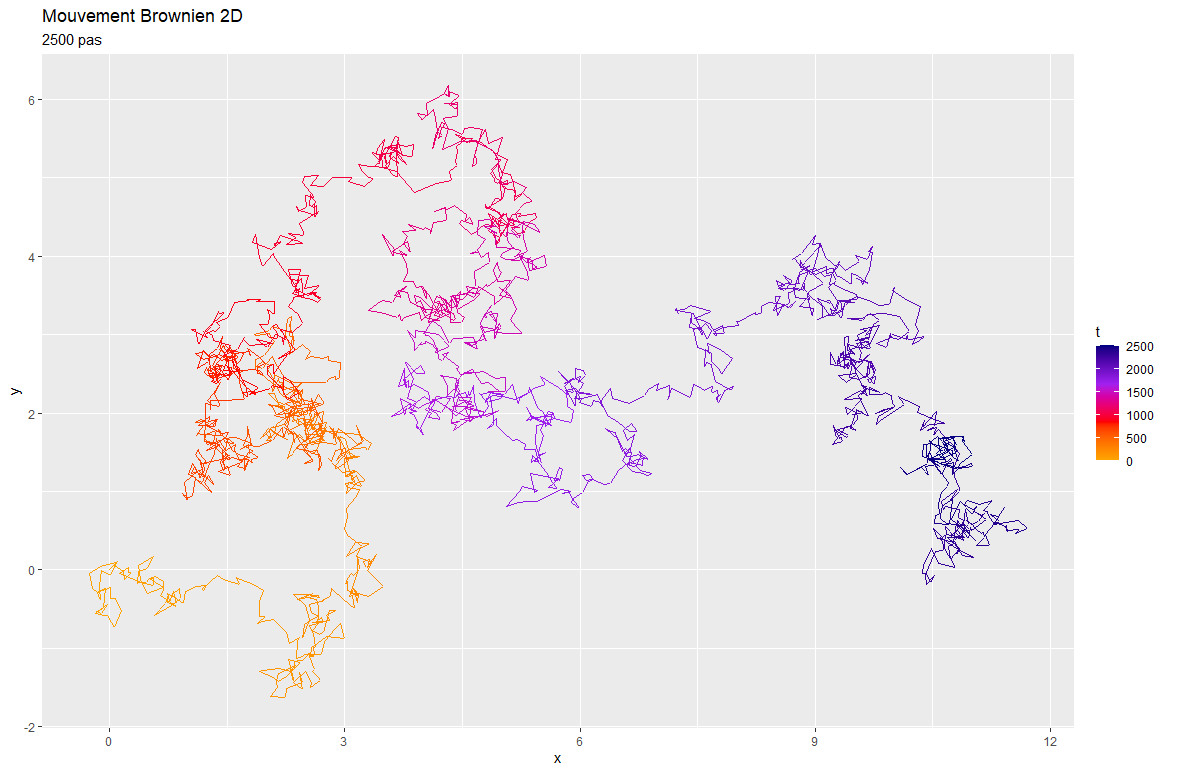
\includegraphics[width=1.1\textwidth]{Images/brownien2D.png}
    \caption{Simulation du mouvement Brownien 2D}
\end{figure}
\vspace{0.03\textheight}
\remarque Le processus de Wiener est continu partout mais dérivable nulle part. Il s'apparente en ce sens à une fonction de Weierstrass.
\vspace{0.025\textheight}\\
Si on considère le déplacement d'une particule dans un espace de dimension $d$, on peut alors associer l'évolution de sa position au processus de Wiener $W_t : \mathbb{\mathbb{R}^+} \to \mathbb{R}^d$. On obtient, de par la nature du mouvement brownien, que la distance moyenne parcourue par la particule jusqu'à $t_\alpha$ vaut $\mathbb{E}[W_t] = 0$ car le mouvement brownien n'a pas de direction privilégiée. \\
Ainsi, on remarque directement que $Var(W_t) = \mathbb{E}[W_t^2]-\mathbb{E}[W_t]^2 = \mathbb{E}[W_t^2]$. \\
On considèrera uniquement les mouvements browniens unidimensionnels par la suite.



On peut également montrer que $W_t$ est un cas particulier de processus stochastique gaussien, c'est-à-dire :
\begin{align*}
    \forall A \subset I, \ \forall (a_t)_{t\in A} \subset \mathbb{R}, \ \ \sum_{s \in A} a_s W_s \sim \mathcal{N}(\mu, \sigma^2) 
\end{align*}

Considérons une option sur un marché. A chaque instant $t$ son prix augmente ou baisse. On peut ainsi modéliser l'évolution du prix d'une option par une marche aléatoire. \\
D'après le \textbf{théorème de Donsker}, cette marche aléatoire converge en loi vers un mouvement brownien standard $W = (W_t, t \geq 0)$. Ainsi, étudier le caractère aléatoire et chaotique de l'évolution du prix d'une option revient à étudier un mouvement brownien.\\

\begin{figure}[H]
    \centering
    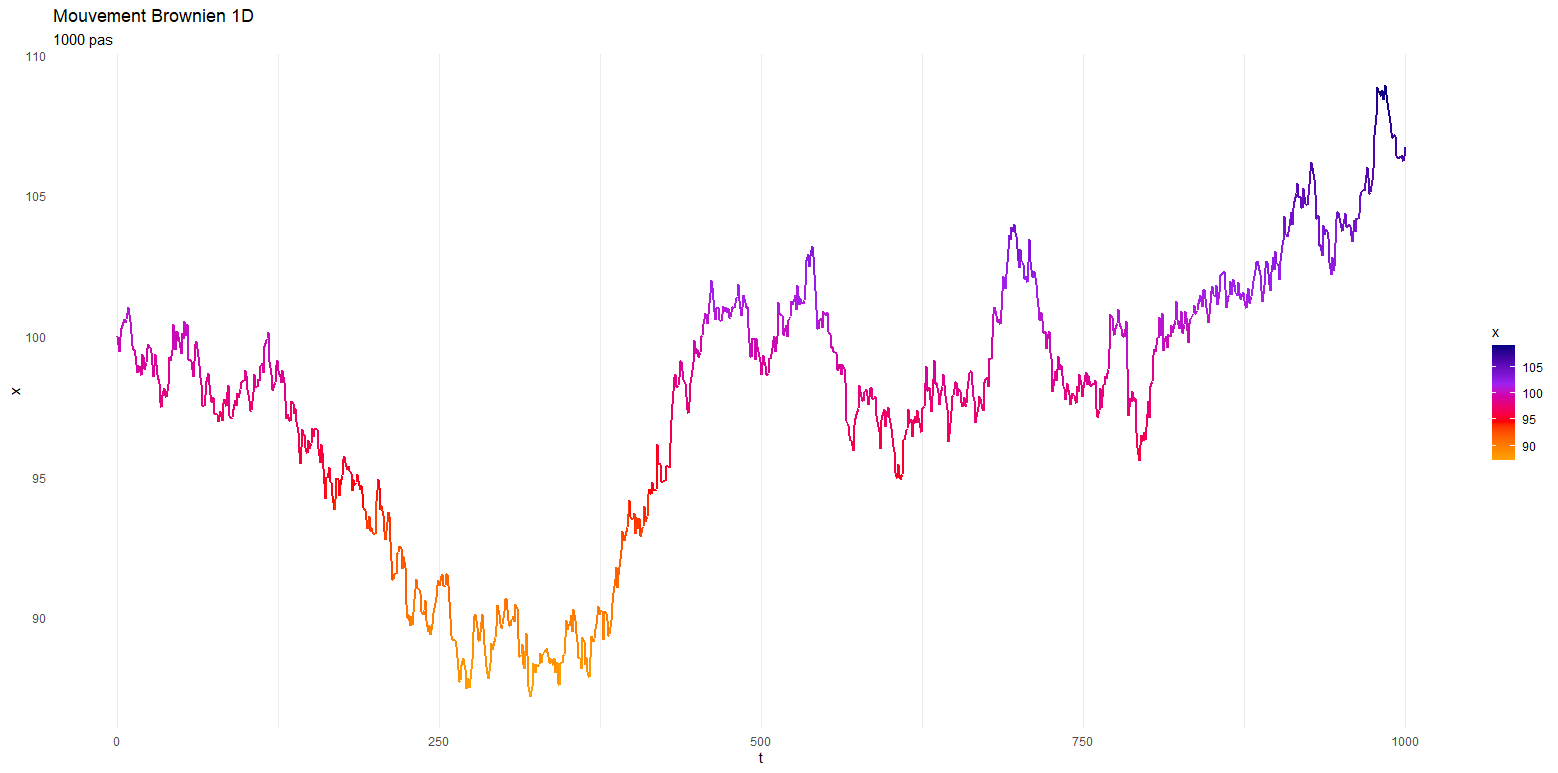
\includegraphics[width=1.1\textwidth]{Images/brownien1D.png}
    \caption{Simulation du mouvement Brownien 1D}
\end{figure}


\subsection{Intégration d'Itō}

Comme vu précédemment,  Il n'existe donc pas de dérivée au sens classique du terme. Le mathématicien Kiyoshi Itō a ainsi développé une nouvelle théorie de l'intégration reposant sur le caractère aléatoire des fonctions à étudier. On va maintenant s'intéresser au calcul des intégrales d'Itō. Ces intégrales permettent d'intégrer des variables aléatoires. L'intégrale est également une variable aléatoire et, en particulier, est une martingale.
\\


On considère un processus de Wiener $W_t$ sur un intervalle $I = [0; T]$ avec $T \in \mathbb{R^+}$ et une subdivision régulière de cet intervalle $0=t_0<t_1<...<t_n=T$, avec $n \in \mathbb{N}$. De manière analogue à l'intégration de Riemann, on peut approcher la valeur de l'intégrale à l'aide de sommes partielles de rectangles de longueur $t_{i+1}-t_i$ et de hauteur $W_t$. Le côté gauche du rectangle doit coïncider avec la valeur à gauche de l'intégrande car le mouvement brownien est une martingale et ne doit pas tenir compte du futur (si l'on prenait le milieu de chaque segment de subdivision, on obtiendrait une intégrale de Stratonovich). Ainsi l'intégrale d'Itō est définie comme la limite en moyenne quadratique de la somme de Riemann évaluée en borne gauche :

\begin{align*}
    I(T) = \int_0^T W_tdW_t &= \lim_{n \to \infty} \sum_{i=0}^{n-1} W_{t_i}(W_{t_{i+1}}-W_{t_i})\\
    \text{en utilisant l'identité }& a(b-a) = \frac{1}{2}(b^2-a^2-(b-a)^2) \text{ avec } a = W_{t_i} \text{ et } b = W_{t_{i+1}}\\
    \implies W_{t_i}(W_{t_{i+1}}-W_{t_i}) &= \frac{1}{2}(W_{t_{i+1}}^2-W_{t_i}^2)-\frac{1}{2}(W_{t_{i+1}}-W_{t_i})^2 \\
    \implies \sum_{i=0}^{n-1} W_{t_i}(W_{t_{i+1}}-W_{t_i}) &= \frac{1}{2}\sum_{i=0}^{n-1}(W_{t_{i+1}}^2-W_{t_i}^2)-\frac{1}{2}\sum_{i=0}^{n-1}(W_{t_{i+1}}-W_{t_i})^2 \\
    \text{or }\sum_{i=0}^{n-1} (W_{t_{i+1}}^2 - W_{t_i}^2) &= W_{t_n}^2 - W_{t_0}^2 = W_T^2 \text{ par somme téléscopique}\\
    \text{et }\sum_{i=0}^{n-1} (W_{t_{i+1}} - W_{t_i})&^2 \xrightarrow{L^2} T \text{ car } \mathbb{E}[(W_{t_{i+1}} - W_{t_i})^2] = Var(W_{t_{i+1}} - W_{t_i}) = t_{i+1} - t_i\\
    \implies I(T) &= \int_0^TW_tdW_t=\frac{1}{2}W_T^2-\frac{1}{2}T\\
\end{align*}

Ainsi, $I(t)$ dépend de deux membres, le premier représentant la position finale quadratique et le second correspond à un ajustement de la volatilité. Sans le dernier terme, l'intégrale ne serait pas une martingale.\\

Terminons notre introduction de ce type d'intégration avec un lemme appelé : \textbf{Lemme d'Itō}.
Il faut ainsi définir le \textbf{processus d'Itō :}
\
$$I_t = \int_0^t \mu_sds+\int_0^t\sigma_sdW_s \quad\text{ qui est équivalent à } \quad dI_t=\mu_tdt+\sigma_tdW_t$$
avec $W_t$ un processus de Wiener, $\mu\in L^1$ et $\sigma\in L^2$ des processus déterministes. \\
\remarque Le processus de Wiener a une espérance nulle donc $\mathbb{E}[I_t]=\int_0^t\mu_sds$ et a une variance non nulle donc $Var[X_t]=\int_0^t\sigma^2dW_s$ \\

\begin{definitionbox}[frametitle = {Lemme d'Itō}]
    Soit $\mu\in L^1$,$\sigma\in L^2$,$I_t$ un processus d'Itō et $f(I_t,t)$ une fonction de classe $\mathcal{C}^2(\mathbb{R \times R^+, R)}$ alors :
    $$d(f(I_t,t))=\dfrac{\partial f}{\partial t}(I_t,t)dt+\dfrac{\partial f}{\partial x}(I_t,t)dI_t+\frac{1}{2}\dfrac{\partial^2 f}{\partial x^2}(I_t,t)\sigma^2_tdt$$
\end{definitionbox}

On a précédemment comparé l'évolution d'une option sur un marché à un mouvement brownien. Cependant, le prix d'une option ne peut pas être négatif. Pour pallier ce problème, on peut définir le \textbf{processus log-normal} ou \textbf{mouvement brownien géométrique} :
$$X_t = X_0e^{(a-\frac{1}{2}\sigma^2)t + \sigma W_t} \quad\text{avec } a,\sigma\in \mathbb{R}$$
Ainsi, on le mouvement brownien géométrique est solution de l'équation différentielle stochastique : $dX_t = a X_t dt + \sigma X_t dW_t$ \\
\proofname{} \\
Soit $X_t = X_0e^{(a-\frac{1}{2}\sigma^2)t + \sigma W_t} \quad\text{avec } a,\sigma\in \mathbb{R}$. On pose alors le processus d'Itō $I_t = (a - \frac{1}{2}\sigma^2)t + \sigma W_t$. \\
On a alors $dY_t = \underbrace{(a - \frac{1}{2}\sigma^2)}_{\mu_t} dt + \underbrace{\sigma}_{\sigma_t} dW_t$ \\
On définit la fonction $f(x, t) = X_0 e^x$ telle que $f(I_t, t) = X_t$
\begin{itemize}
    \item $\dfrac{\partial f}{\partial t}(I_t, t)=0$
    \item $\dfrac{\partial f}{\partial x}(I_t, t)=X_0e^{I_t}=X_t$
    \item $\dfrac{\partial^2 f}{\partial x^2}(I_t, t)=X_0e^{I_t}=X_t$
\end{itemize}
On peut alors appliquer le lemme d'Itō:
$$dX_t = 0 \cdot dt + X_tdI_t+\dfrac{1}{2}X_t\sigma^2dt$$
Substituons $dI_t$ par $(a - \frac{1}{2}\sigma^2)dt + \sigma dW_t$ :
\begin{align*}
    dX_t &= X_t[(a - \frac{1}{2}\sigma^2)dt + \sigma dW_t]+\dfrac{1}{2}X_t\sigma^2dt \\
    &= aX_tdt - \frac{1}{2}\sigma^2X_tdt +\sigma X_tdW_t+\dfrac{1}{2}X_t\sigma^2dt \\
    &=aX_tdt+\sigma X_tdW_t
\end{align*}
Finalement, on a bien : 
$$dX_t = a X_t dt + \sigma X_t dW_t$$ \\

Après avoir défini tous ces processus, nous allons pouvoir les appliquer au modèle de Black-Scholes dans la sous-partie suivante.
\subsection{Equation de Black-Scholes}
Introduisons maintenant l'équation aux dérivées partielles la plus importante des mathématiques financières : l'équation de Black-Scholes dont le nom fait référence à Fischer Black et Myron Scholes qui l'ont évoqué dans un texte de recherche académique. Nous allons étudier le modèle de Black-Scholes dans un premier temps avant de montrer qu'en diminuant les pas de temps, le modèle de cox-Ross-Rubinstein converge vers le modèle de Black-Scholes.

\vspace{0.05\textheight}
\begin{definitionbox}[frametitle = {Equation aux Dérivées Partielles de Black-Scholes}]
    Soit $V(S,t)$ le prix d'une option avec $S$ le prix du sous-jacent et $t$ représentant le temps :
    $$\frac{\partial V}{\partial t} + \frac{1}{2}\sigma^2S^2\frac{\partial^2V}{\partial S^2}+rS\frac{\partial V}{\partial S}-rV=0$$
\end{definitionbox}
\vspace{0.05\textheight}
Le modèle repose sur un grand nombre d'hypothèses assez contraignantes, nécessaires pour la démonstration de la formule. Le but étant d'étudier le modèle de Cox-Ross-Rubinstein. Je vais donner les hypothèses simplifiées nécessaires à la compréhension de la résolution. Elles sont néanmois trouvables sur \hyperlink{https://fr.wikipedia.org/wiki/Modèle_Black-Scholes}{la page Wikipédia du modèle de Black-Scholes}. 
\vspace{0.025\textheight}\\
Les hypothèses de ce modèle sont donc : 
\begin{itemize}
    \item Le taux sans risque est constant
    \item Le prix suit un mouvement brownien géométrique et la variance du mouvement est constante
    \item L'option ne donne pas de dividende
    \item Le marché respecte l'AOA
    \item Le marché permet de vendre un actif en n'importe quelle quantité
    \item Les transactions n'occasionnent aucun frais
\end{itemize}
\vspace{0.025\textheight}
La formule de Black-Scholes permet de calculer le prix d'un \textbf{call ou put européen} mais ne permet pas de calculer des calls/puts américains contrairement au modèle de Cox-Ross-Rubinstein.

\subsection{Convergence}
\newpage
\section{Evaluations des indicateurs de risque}

Dans cette partie, nous nous intéresserons dans un premier temps à la théorie entourant les indicateurs de risque, appelés \textbf{Grecques}, puis nous utiliserons le modèle binomial pour essayer de les approximer. Nous nous limiterons ici aux grecques principales : $\Delta, \Gamma, \nu, \Theta$. Il en existe de nombreuses autres, notamment $\rho, \lambda, \epsilon$, mais qui sont moins pertinentes en raison des hypothèses présupposées du modèle binomial (taux sans risque constant, pas de dividende, etc.).

\subsection{Delta $(\Delta)$}

\subsection{Gamma $(\Gamma)$}

\subsection{Vega $(\nu)$}

\subsection{Thêta $(\Theta)$}
\newpage
\section{Analyse comparative avec d'autres modèles}

\subsection{Monte-Carlo}

\subsection{Arbres trinomiaux}

\subsection{???}

\subsection{???}
\newpage
\input{partie8}
\newpage
\begin{center}
    \rule{\textwidth}{1pt} \\[0.5cm]
    {\Huge \bfseries ANNEXES} \\[0.4cm]
    \rule{\textwidth}{1pt}
\end{center}


\section*{Code R pour simuler un mouvement brownien 2D}
\begin{verbatim}
    library(ggplot2)
    
    n <- 2500
    dt <- 0.01

    df <- data.frame(
        x = cumsum(c(0, rnorm(n, 0, sqrt(dt)))),
        y = cumsum(c(0, rnorm(n, 0, sqrt(dt)))),
        t = 0:n
    )

    ggplot(df, aes(x, y, color = t)) + geom_path() +
    scale_color_gradientn(colors = c("orange", "red", "purple", "navy")) +
    coord_fixed() + labs(title = "Mouvement Brownien 2D", subtitle = paste(n, "pas"))
\end{verbatim}

\section*{Code R pour simuler un mouvement brownien 1D}
\begin{verbatim}
    library(ggplot2)
    
    n <- 1000 
    dt <- 0.0001 
    
    df <- data.frame(
        x = cumsum(c(100, rnorm(n, 0, 0.5))),
        t = 0:n
    )
    
    ggplot(df, aes(t, x, color = x)) + geom_line(linewidth = 1) + 
        scale_color_gradientn(colors = c("orange", "red", "purple", "navy")) + 
        coord_cartesian(xlim = c(0, n)) + theme_minimal() +
        theme(panel.grid.major.y = element_blank(), panel.grid.minor.y = element_blank()) +
        labs(title = "Mouvement Brownien 1D", subtitle = paste(n, "pas"))
\end{verbatim}


  

\newpage
\printbibliography

\end{document}